\noindent{\textbf{Failure case analysis.}} A qualitative analysis of segmentation performance on the test set in~\cref{fig:fail-anal} reveals that SS-JEPA struggles with landslides of small spatial extent. In terms of mIoU, I-JEPA exceeds SS-JEPA in (emprirically) 85\% of cases by a margin of 0.005 to 0.3. This stems from a bias toward broad patterns in SS-JEPA, where the large number of patch tokens allows background data to overwhelm sharp, localized details. The linear projection layer acts as a bottleneck that favors this broad consensus, effectively smoothing out high-frequency spatial signals during fusion. While I-JEPA’s early fusion preserves these details, SS-JEPA’s integration tends to suppress features with limited spatial spread. Future work will focus on adaptive weighting to protect localized signals against such bias.

\begin{figure}
	\begin{center}
		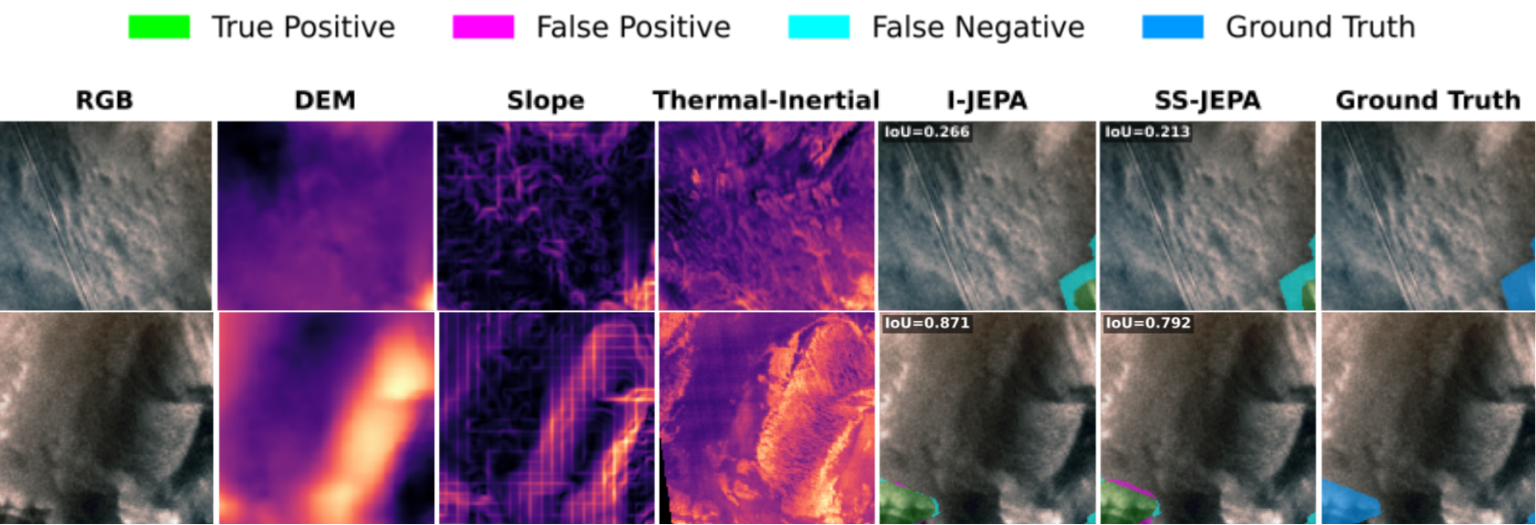
\includegraphics[width=0.95\linewidth]{figures/qual-plots-failure-anal.png}
	\end{center}
	\vspace{-1.5em}
	\caption{Qualitative analysis of failure cases of SS-JEPA}\label{fig:fail-anal}
	\vspace{0.5em}
\end{figure}

\noindent{\textbf{Original UPerNet comparison.}} As requested, for fairer comparison we have reported metrics for the original UPerNet with a ViT backbone as a baseline in~\cref{tab:decoders}.

\begin{table}
	\centering
	\scriptsize % Reduces font size to save space
	\setlength{\tabcolsep}{3pt} % Tightly packs the columns
	\vspace{-1.5em}
	\caption{Segmentation Decoder Performance with ViT encoder. Standard deviation (SD) taken over 5 runs}
	\label{tab:decoders}
	\begin{tabular}{lcccccc}
		\toprule
		\textbf{Model} & \textbf{mIoU} & \textbf{Precision} & \textbf{Recall} & \textbf{F1 Score} & \textbf{FG IoU} & \textbf{BG IoU} \\
		\midrule
		UPerNet        & 0.8210        & 0.8670             & 0.8710          & 0.8690            & 0.7690          & 0.8730          \\
		\bottomrule
	\end{tabular}
	\vspace{-1.5em}
\end{table}


\noindent\textbf{Single dataset / incremental gain / two-stage overhead.} We
already note the 5.6$\times$ parameter reduction over the ensemble (Sec.~4.4)
as the practical trade-off for the 0.2\% gap; MMLSv2 is, to our knowledge,
the only public multimodal Mars landslide segmentation benchmark, which we state
explicitly as a limitation in Sec.~5.

\noindent\textbf{Mars-related literature.} Thank you for the pointers -- we will add a discussion of [1--3] from the reviewer comments to Sec.~2.1 in the camera-ready version.

